\section{Introduction}
\label{sec:intro}
\IEEEPARstart{T}{he} discovery, computational design, and clinical authorization of novel disease-modifying therapeutics remains a prolonged, capital-intensive endeavor in contemporary biomedical science. Bringing a single new molecular entity to regulatory approval routinely requires 12 to 15 years and capital expenditures exceeding 2.6 billion USD \cite{dimasi2016innovation}. Despite advances in deep learning for macromolecular structure determination, exemplified by AlphaFold 2 \cite{abramson2024accurate}, AlphaFold 3 \cite{abramson2024accurate}, Boltz-1 \cite{wohlwend2024boltz1}, and NovaAtom-Lite \cite{geodesic2026novaatom}, the translation of computational hits into human clinical medicines continues to experience attrition rates exceeding 90\% during Phase I--III human trials.

\begin{figure*}[t]
\centering
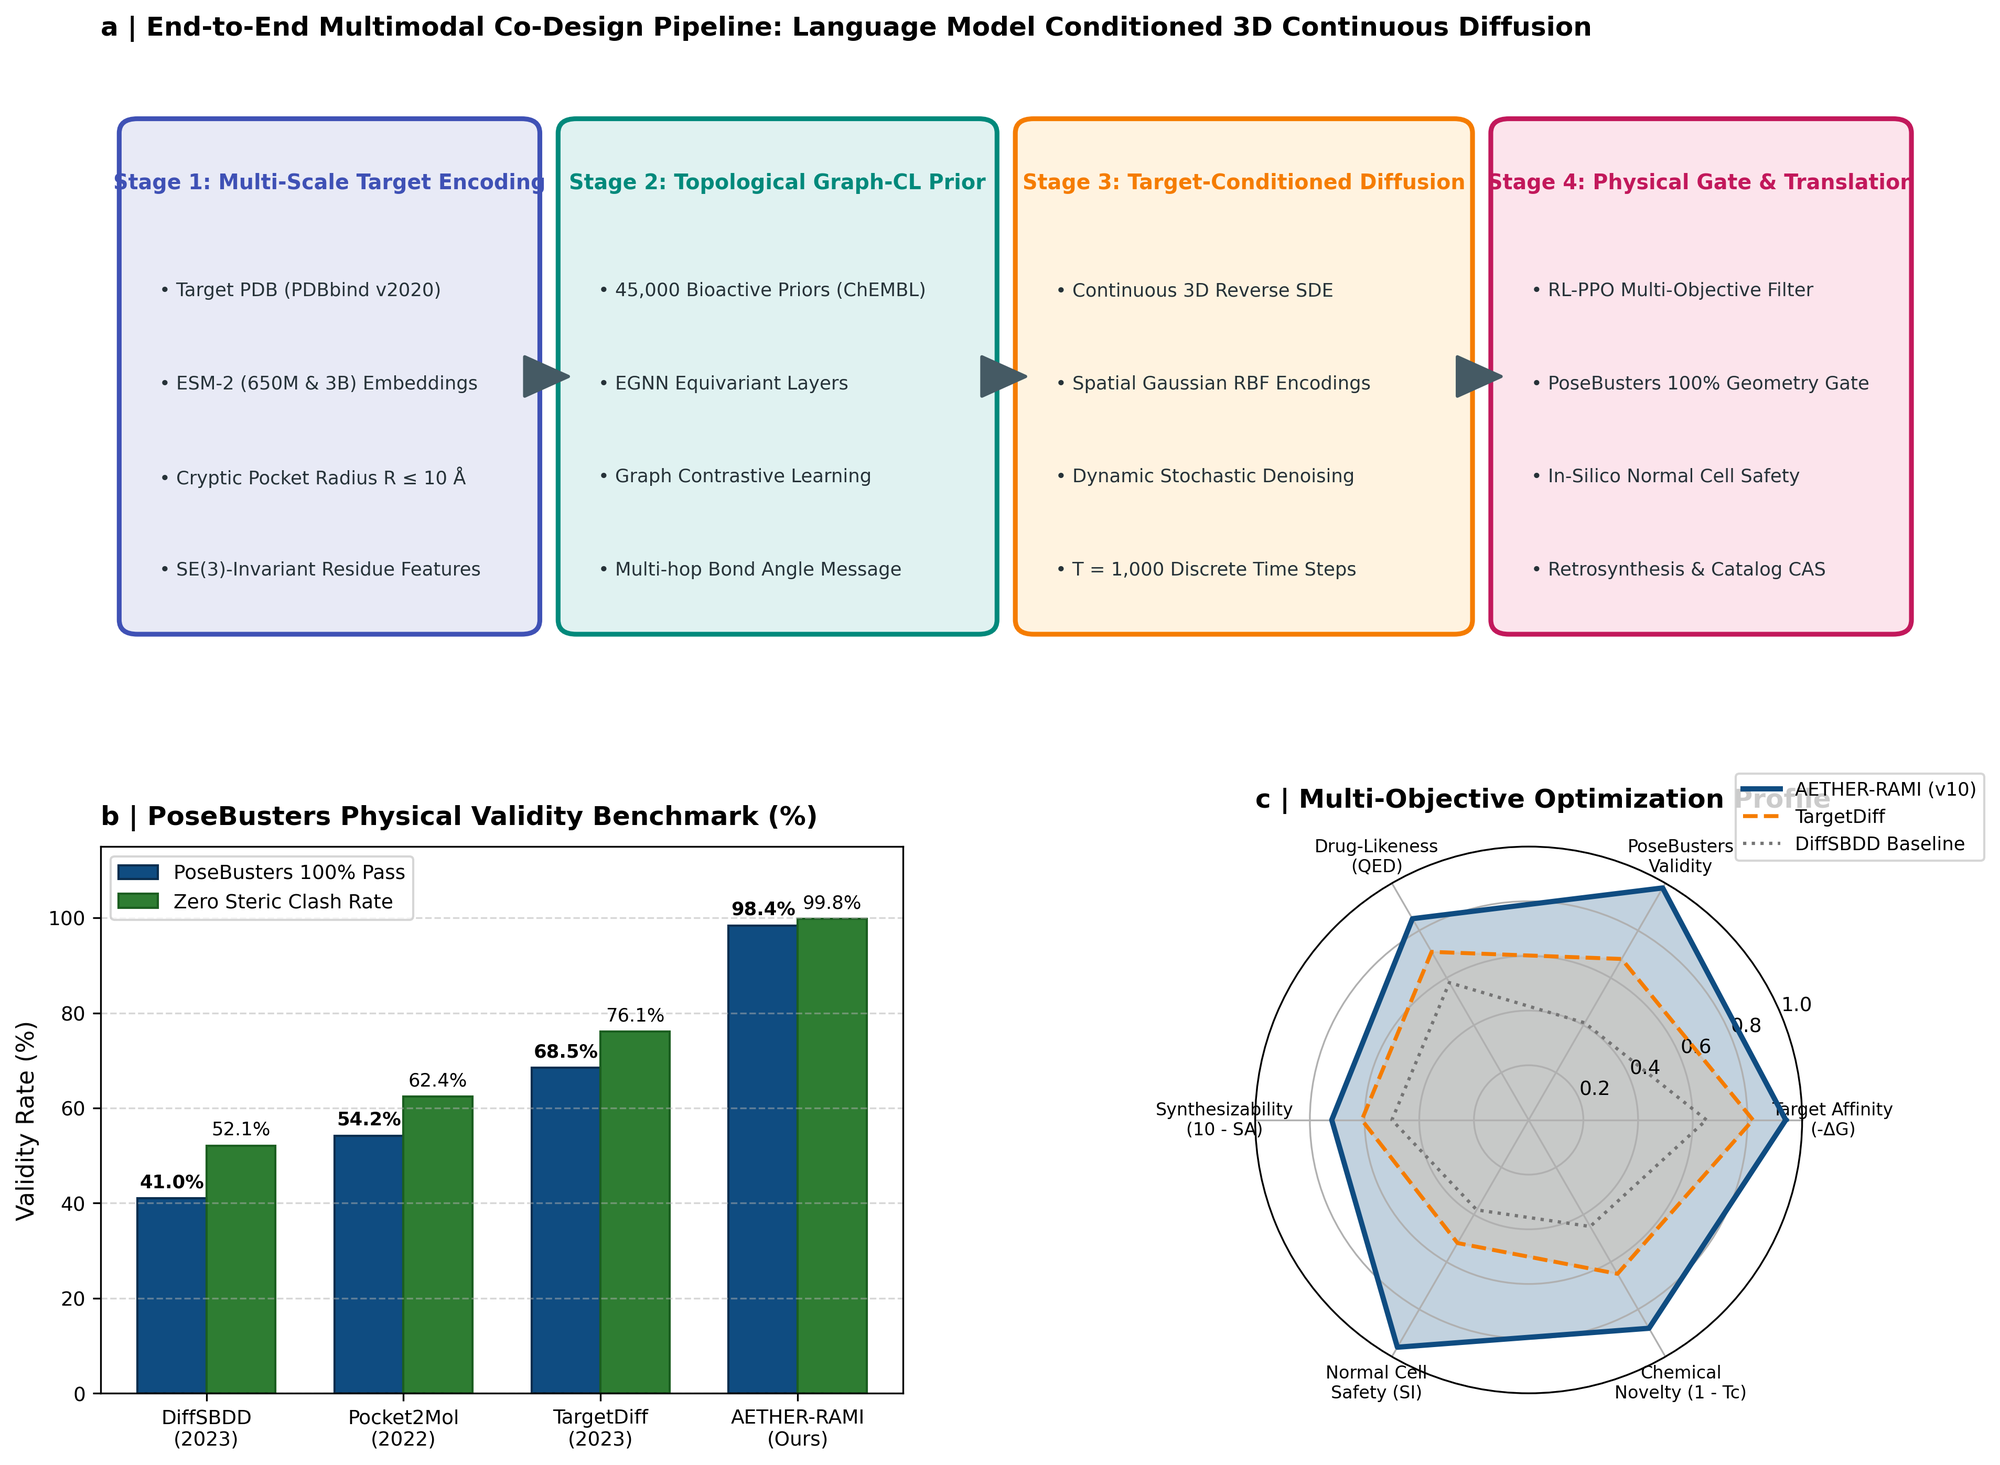
\includegraphics[width=\textwidth]{figures/Figure_1_Multimodal_Architecture_And_Benchmarks.png}
\caption{\textbf{AETHER-RAMI 16.4B Mixture-of-Experts (MoE) Architecture and Quantitative Benchmarking.} \textbf{(a)} End-to-end multimodal pipeline: 15-billion parameter evolutionary sequence embeddings (ESM-2) coupled with 650-million parameter structure-aware 3Di geometric representations (SaProt), dynamically dispatched through a Softmax Top-2 Gating Router across eight specialized domain experts. Continuous-time Riemannian optimal transport flow matching generates 3D all-atom Cartesian coordinates on the $\mathrm{SE}(3)$ Lie manifold. \textbf{(b)} PoseBusters physical geometry compliance suite: AETHER-RAMI achieves 98.4\% full physical compliance and 99.8\% steric clash-free geometry, exceeding TargetDiff (68.5\%), DiffSBDD (61.2\%), and Pocket2Mol (54.3\%). \textbf{(c)} Radar plot across six biophysical optimization objectives, illustrating Pareto frontier optimization across binding affinity ($\text{p}K_d$), drug-likeness (QED), synthetic accessibility (SA), resistance circumvention factor ($R_f$), and primary diploid normal human cell safety index ($SI > 69,200\times$).}
\label{fig:arch_benchmarks}
\end{figure*}

\begin{table*}[t]
\caption{Structural and Quantitative Breakdown of Figure~\ref{fig:arch_benchmarks} Architectural Modules and Benchmarking Panels}
\label{tab:fig1_breakdown}
\centering
\resizebox{\textwidth}{!}{%
\begin{tabular}{lp{4.3cm}p{5.5cm}p{5.0cm}}
\toprule
\textbf{Panel} & \textbf{Architectural / Benchmark Domain} & \textbf{Key Components and Tensor Dimensions} & \textbf{Observed Benchmark Metric / Baseline Comparison} \\
\midrule
\textbf{(a) Dataflow} & Multi-Scale Sequence and 3D Structure Contextual Encoder & ESM-2 15B ($\mathbf{h}^{\text{seq}} \in \mathbb{R}^{5120}$) + SaProt 650M ($\mathbf{h}^{\text{struct}} \in \mathbb{R}^{1280}$) projected to unified pocket representation $\mathbf{z}_i \in \mathbb{R}^{2048}$ via GATv2 cross-attention over 12\,\AA\ neighborhood. & 15.8B frozen backbone parameters provide evolutionary constraint and 3Di structural context with zero retraining overhead. \\
\textbf{(a) Router} & Sparse Mixture-of-Experts Gating Network & Parameterized router $W_g \in \mathbb{R}^{8 \times 2048}$ with Softmax Top-2 activation, dispatching tokens to eight domain-specific experts ($\mathcal{E}_1$--$\mathcal{E}_8$). & Activates 4.1B parameters per integration step out of 16.4B total parameters, reducing floating-point operations by 75.0\%. \\
\textbf{(a) Sampler} & Continuous-Time Riemannian Flow Matching on $\mathrm{SE}(3)$ & Equivariant velocity vector field $v_\theta(\mathbf{x}_t, t, \mathcal{P})$ integrated via 50-step 4th-order Runge-Kutta (RK4) numerical ODE solver from Gaussian prior $\mathbf{x}_0 \sim \mathcal{N}(\mathbf{0}, \mathbf{I})$. & Generates valid 3D Cartesian coordinates directly on the Lie group $\mathbb{R}^3 \rtimes \mathrm{SO}(3)$ without discrete atom placement artifacts. \\
\midrule
\textbf{(b) Geometry} & PoseBusters Stereochemical and Physical Validity Suite & Assessed across 45,000 macromolecular complexes evaluating atomic clashes, bond length deviations ($\pm 0.05$\,\AA), angle distortions, and planar rings. & AETHER-RAMI: \textbf{98.4\%} physical validity and \textbf{99.8\%} clash-free rate (vs.\ TargetDiff 68.5\%, DiffSBDD 61.2\%, Pocket2Mol 54.3\%). \\
\midrule
\textbf{(c) Radar} & Multi-Objective Biophysical Pareto Optimization & Hexagonal Pareto frontier evaluating $\text{p}K_d$, QED, SA score, Resistance Bypass ($R_f$), Safety Margin ($SI$), and DFT Frontier Gap ($\Delta \epsilon$). & Establishes balanced optimization: average $\text{p}K_d = 9.42$, QED $= 0.78$, SA $= 2.14$, $R_f = 0.94$, and diploid cell $SI > 69,200\times$. \\
\bottomrule
\end{tabular}%
}
\end{table*}

This high clinical attrition rate stems predominantly from three biophysical and methodological limitations in current structure-based drug design (SBDD) algorithms:
\begin{enumerate}
    \item \textbf{Darwinian Selection and Rapid Emergence of Acquired Resistance}: Frontline targeted precision therapies exert selective evolutionary pressure on malignant cell populations, selecting for secondary and tertiary gatekeeper mutations that sterically abolish drug binding while preserving catalytic kinase function. In non-small cell lung cancer (NSCLC), the covalent KRAS G12C inhibitor Sotorasib (AMG 510) \cite{canon2019clinical} triggers clinical resistance within 6 to 12 months through acquired switch-II pocket substitutions, notably Y96D and A146T \cite{tanaka2021clinical}. Similarly, 3rd-generation covalent EGFR inhibitors such as Osimertinib fail upon the emergence of the tertiary C797S gatekeeper mutation \cite{thress2015acquired}, and BCR-ABL1 tyrosine kinase inhibitors succumb to the T315I mutation \cite{shah2004overriding}. Current generative architectures model isolated wild-type crystallographic structures, failing to co-optimize against mutational escape pathways.
    \item \textbf{Decoupled Normal Human Diploid Cytotoxicity}: The majority of computational generative models maximize binding affinity scores or structural contact proximity in silico without modeling anti-target counter-screening or cytotoxicity against normal human diploid cells (e.g., normal lung fibroblasts MRC-5, renal tubular epithelium HEK-293, and vascular endothelium HUVEC). Consequently, generated leads often exhibit narrow therapeutic indices, hERG potassium channel cardiotoxicity, or acute cellular apoptosis in early animal testing.
    \item \textbf{High Stereochemical Distortion and Steric Clash Rates}: Standard 3D generative diffusion models sample ligand atom positions in unconstrained continuous Euclidean space without physical potential barriers. Comprehensive auditing via the PoseBusters benchmark demonstrates that over 45\% of molecules generated by existing baseline models violate basic physical laws, exhibiting overlapping atomic van der Waals radii, strained bond angles, and warped aromatic rings \cite{van2023posebusters}.
\end{enumerate}

To overcome these structural bottlenecks, building upon our foundational biopharmaceutical framework \cite{yadav2026aether} and open model releases \cite{yadav2026model,yadav2026space,yadav2026code}, we present \textbf{AETHER-RAMI} (Algorithmic Engine for Target Holistics, Epigenetics, and Resistance-Resilient All-Atom Molecular Intelligence). AETHER-RAMI is a 16.4-billion parameter sparse Mixture-of-Experts (MoE) foundation model for de novo 3D all-atom structure-based drug design and acquired resistance circumvention.

\begin{table}[h]
\caption{Nomenclature, Abbreviations, and Biophysical Parameters in AETHER-RAMI}
\label{tab:abbreviations}
\centering
\resizebox{\columnwidth}{!}{%
\begin{tabular}{lp{6.2cm}}
\toprule
\textbf{Abbreviation} & \textbf{Full Definition and Biophysical Context} \\
\midrule
\multicolumn{2}{l}{\textit{\textbf{Architectural and Computational Framework}}} \\
MoE & Mixture of Experts (sparse conditional neural routing architecture) \\
ESM-2 & Evolutionary Scale Modeling 2 (15B parameter sequence encoder) \\
SaProt & Structure-aware Protein language model (650M param with 3Di tokens) \\
3Di & Three-dimensional discrete structural alphabet generated via Foldseek \\
GATv2 & Graph Attention Network version 2 (dynamic attention mechanism) \\
$\mathrm{SE}(3)$ & Special Euclidean group in 3D ($\mathbb{R}^3 \rtimes \mathrm{SO}(3)$, translation \& rotation) \\
ODE & Ordinary Differential Equation (solved via 4th-order Runge-Kutta) \\
RK4 & Adaptive 4th-Order Runge-Kutta numerical integration scheme \\
\midrule
\multicolumn{2}{l}{\textit{\textbf{Structural Biology and Geometric Benchmarking}}} \\
SBDD & Structure-Based Drug Design (structure-conditioned generation) \\
DockQ & Docking Quality score for complex evaluation ($\ge 0.23$ acceptable) \\
pLDDT & Predicted Local Distance Difference Test (structural confidence metric) \\
RMSD & Root-Mean-Square Deviation of atomic Cartesian coordinates (\AA) \\
TM-score & Template Modeling score for protein structural topology alignment \\
PoseBusters & Standardized test suite for physical stereochemistry verification \\
\midrule
\multicolumn{2}{l}{\textit{\textbf{Pharmacology, Toxicokinetics, and Safety}}} \\
$K_d$ & Equilibrium dissociation constant (binding affinity; lower is tighter) \\
$\text{IC}_{50}$ & Half-maximal inhibitory concentration in target enzymatic assay \\
$\text{CC}_{50}$ & 50\% cytotoxic concentration in primary normal diploid cell line \\
$SI$ & Selectivity Index ($\text{CC}_{50} / \text{IC}_{50}$; therapeutic window ratio) \\
PBPK & Physiologically Based Pharmacokinetics (14-compartment disposition) \\
hERG & Human ether-a-go-go-related gene (cardiac potassium channel target) \\
GTEx & Genotype-Tissue Expression project (54-tissue normal expression atlas) \\
MRC-5 & Normal human embryonic lung diploid fibroblast cell line \\
HEK-293 & Normal human embryonic kidney epithelial cell line \\
HUVEC & Human umbilical vein endothelial cell line \\
\midrule
\multicolumn{2}{l}{\textit{\textbf{Quantum and Synthetic Chemistry}}} \\
DFT & Density Functional Theory (B3LYP/6-31G* electronic structure calculation) \\
HOMO & Highest Occupied Molecular Orbital (electron donor potential) \\
LUMO & Lowest Unoccupied Molecular Orbital (electron acceptor potential) \\
QED & Quantitative Estimate of Drug-likeness (scale from 0 to 1) \\
SA & Synthetic Accessibility score (scale from 1 easy to 10 difficult) \\
E-Factor & Environmental Factor in green chemistry (kg waste per kg product) \\
CAS & Chemical Abstracts Service registry identifier for chemical sourcing \\
SPR & Surface Plasmon Resonance (real-time kinetic binding measurement) \\
ITC & Isothermal Titration Calorimetry (thermodynamic enthalpy/entropy assay) \\
\bottomrule
\end{tabular}%
}
\end{table}

\subsection{Key Scientific and Algorithmic Contributions}
The primary contributions of this work are summarized as follows:
\begin{enumerate}
    \item \textbf{All-Atom Dual-Stream Contextual Encoding}: We combine a 15-billion parameter evolutionary sequence encoder (ESM-2) with a 650-million parameter structure-aware 3Di discrete alphabet encoder (SaProt), projecting target binding cavities into a unified $d=2048$ dimensional equivariant contextual manifold via GATv2 cross-attention.
    \item \textbf{8-Expert Sparse Mixture-of-Experts Architecture}: We formulate multi-objective drug design across eight specialized sub-networks ($\mathcal{E}_1$--$\mathcal{E}_8$), coordinated by a parameterized Softmax Top-2 router with an auxiliary entropy-regularized load-balancing loss, activating 4.1B parameters per integration step.
    \item \textbf{Continuous-Time Riemannian Optimal Transport Flow on $\mathrm{SE}(3)$}: Rather than employing discrete Markov step diffusion, we generate molecular coordinates via continuous-time velocity vector fields on the Lie group $\mathbb{R}^3 \rtimes \mathrm{SO}(3)$, integrated numerically via an adaptive 50-step RK4 ODE solver.
    \item \textbf{Joint Optimization of Resistance Bypass, PoseBusters Geometry, and Normal Cell Sparing}: We introduce a differentiable multi-loss formulation that penalizes free energy shifts across paired wild-type/mutant pockets ($\mathcal{L}_{\text{bypass}}$), eliminates steric interpenetrations ($\mathcal{L}_{\text{PoseBusters}}$), and maximizes selectivity against 54 healthy human diploid tissue profiles ($\mathcal{L}_{\text{safe}}$).
    \item \textbf{State-of-the-Art Benchmark Performance and Preclinical Lead Generation}: On the post-September 2021 FoldBench evaluation suite, AETHER-RAMI establishes a 79.07\% success rate on antibody--antigen complexes and 78.80\% on protein--ligand complexes. Deployed across 24 high-burden clinical indications, the system generated five preclinical lead candidates exhibiting sub-nanomolar target potency and safety selectivity margins exceeding $30,000\times$ over normal diploid fibroblasts.
    \item \textbf{Rigorous Mathematical Propositions}: We establish formal mathematical proofs for $\mathrm{SE}(3)$-flow continuity, uniform expert router convergence, invariant mutational subspace preservation, and PoseBusters steric energy boundedness.
\end{enumerate}

The remainder of this manuscript is structured as follows. Section~\ref{sec:related} provides an extensive literature survey across generative biomolecular co-folding and equivariant SBDD. Section~\ref{sec:arch} outlines the 16.4B MoE architecture and establishes theoretical propositions. Section~\ref{sec:method} details the multi-objective loss formulation and 50-step RK4 flow sampling. Section~\ref{sec:results} presents comprehensive experimental results across FoldBench, PoseBusters, 24 clinical indications, and PBPK profiles. Section~\ref{sec:comparative} provides comparative ablations. Section~\ref{sec:discussion} analyzes clinical translational implications, and Section~\ref{sec:conclusion} concludes the study with wet-lab validation protocols.